\section{奥伯斯佯谬和宇宙的膨胀}\label{sec:05.04}

上节求得的速度分布解,哪一种符合实际情况?我们可以用
所谓奥伯斯(Olbers)佯谬来判定。
\begin{figurex}
    \centering
    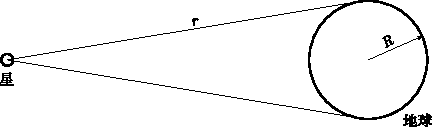
\includegraphics{figure/fig05.02}
    \caption{星体射向地球的光子}
    \label{fig:05.02}
\end{figurex}

奥伯斯佯谬讨论星体发射的光子到达地球的数目。如图\ref{fig:05.02}~,
假定一颗星离地球的距离为$ r $,这颗星每单位时间向四面八方均
匀地发射$ E $个光子。那么,单位时间里落到地球上的光子数应当
等于
\begin{equation}\label{eqn:05.04.01}
    E \frac { \uppi R ^ { 2 } } { 4 \uppi r ^ { 2 } } = \frac { E R ^ { 2 } } { 4 r ^ { 2 } }
\end{equation}
其中$ R $是地球的半径。

\begin{wrapfigure}[8]{r}{14em}
    \centering
    \vspace{-2.5em}
    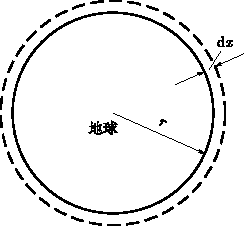
\includegraphics{figure/fig05.03}
    \caption{球壳内星体向地球发射的光子}
    \label{fig:05.03}
\end{wrapfigure}
如图\ref{fig:05.03},考虑一个以地球为中心,$ r $为半径的球壳,它
的厚度为$ \dif r $,这个球壳的体积为
%{\setlength\mathindent{4em}
\begin{equation*}
    4 \uppi r ^ { 2 } \dif r
\end{equation*}%}
如果每单位体积中平均有$ N $个
星体,则球壳内的星体数是
\begin{equation}\label{eqn:05.04.02}
    N  4  \uppi r ^ { 2 } \dif r
\end{equation}
% 160.jpg
因此,在单位时间里地球从这球壳内里体所得到的光子数为
\begin{equation*}
    \dif L = \frac { E R ^ { 2 } } { 4 r ^ { 2 } } N 4 \uppi r ^ { 2 } \dif r
\end{equation*}
这样,整个宇宙中的星体单位时间里射到地球上的光子总数为
\begin{equation}\label{eqn:05.04.03}
    \begin{aligned}
    L &= \int \dif L = \int _ 0 ^ { \infty } { E R ^ { 2 } N \uppi \dif r } \\
      &= \left( E R ^ { 2 } N \right) \uppi \int _ 0 ^ { \infty } \dif r \longrightarrow \infty
    \end{aligned}
\end{equation}
这表明,从地球上看到的天空是无限亮的,而且无论哪个方向上
都是无限亮的。这显然不符合实际情况:夜晚的天空是黑的,白
天的天也并不是无限亮。这个矛盾就称为奥伯斯佯谬。

奥伯斯佯谬说明,在推导式\eqref{eqn:05.04.03}中,我们必定使用了某
个错误的假定。检查一下推导式\eqref{eqn:05.04.03}的过程,我们使用过以
下几个假定:

(1)星体占据的空间是无限的,星体均匀地分布在无限的空
间上;

(2)星体存在的时间是无限的,无论在多久之前都有星体充
满着无限空间,而且,每颗星的平均光度(即每单位时间发射的
光子数)都是$ E $;

(3)整个星体体系没有运动,即各处的星体相互之间保持着
静止。

可见,如果我们采取静止解,则不可能解决奥伯斯佯谬。

如果取宇宙膨胀解或收缩解,则相当于放弃上述的第三条假
定。膨胀解和收缩解对奥伯斯佯谬有什么影响呢?严格地说,这
个问题已不能在牛顿力学的框架内加以讨论,因为在第二章中已
经证明,光是不满足牛顿运动学中的速度合成律式\lhbrak \eqref{eqn:02.03.06}\rhbrak  的。

在本章中,我们将严格按照牛顿力学进行分析,因此,我们
仍认为光也遵从牛顿的速度合成律。这样,对于膨胀解,位于$ r $
% 161.jpg
的星体向地球发射的光的速度为
\begin{equation}\label{eqn:05.04.04}
    c - q = c - | f \left( t \right) | r
\end{equation}
收缩解为
\begin{equation}\label{eqn:05.04.05}
    c - q = c + | f \left( t \right) | r
\end{equation}
如果利用式\eqref{eqn:05.04.05},则式\eqref{eqn:05.04.03}的推导不变,因为所有星光仍
都能到达地球。所以,收缩解也不能解决奥伯斯佯谬。

若取式\eqref{eqn:05.04.04},则看到,对于
\begin{equation*}
    r \geqslant \frac { c } { | f \left( t \right) | }
\end{equation*}
的天体,其光子速度变为负值,亦即这种光子的速度并不是向着
地球,而是背向地球,故这种光子永远不能到达地球。这时,式
\eqref{eqn:05.04.03}中的积分限应改成从0到$  c / | f \left( t \right) |   $,积分可成为有限。所
以,膨胀解可以解决奥伯断佯谬。

总之,从哥白尼原理出发,在牛顿力学的框架内,我们证明
了宇宙必定在膨胀。

1930年以来,天文观测直接证实了这个结果:宇宙在膨胀。
的确发现,星体相对于我们的膨胀速度正比于它的距离,符合式
\eqref{eqn:05.04.05} 。测得
\begin{equation}\label{eqn:05.04.06}
    | f \left( t _ { 0 } \right) | \equiv H _ { 0 } \approx 15 \text{千米/(秒\ensuremath{\cdot}百万光年) }
\end{equation}
即相距我们一百万光年的天体,逃离我们的速度为15千米/秒。
上式中的$ t _ 0 $表示现在的时刻。
